\documentclass[11pt,a4paper]{article}
\usepackage[utf8]{inputenc}
\usepackage{amsmath, mathtools}
\usepackage{amsfonts, dsfont}
\usepackage{amssymb}
\usepackage{graphicx}
\usepackage{empheq}
\usepackage{bm}
\usepackage[round, sort]{natbib}
\usepackage{tikz}
\usepackage{mathtools}  
%\mathtoolsset{showonlyrefs}  
\usetikzlibrary{shapes,backgrounds,arrows,automata,snakes,shadows,positioning, mindmap}

%%%%% Commands
\newtheorem{theorem}{Theorem}
\newtheorem{lemma}{Lemma}
\newcommand{\argmin}{\arg\!\min}
\newcommand{\argmax}{\arg\!\max}
\newcommand*\widefbox[1]{\fbox{\hspace{3em}#1\hspace{3em}}}
\newcommand*\lesswidefbox[1]{\fbox{\hspace{2em}#1\hspace{2em}}}
\newcommand{\entr}{\mathcal{H}}
\newcommand{\betabf}{\boldsymbol{\beta}}
\newcommand{\thetabf}{\boldsymbol{\theta}}
\newcommand{\mubf}{\boldsymbol{\mu}}
\newcommand{\Omegabf}{\boldsymbol{\Omega}}
\newcommand{\Sigmabf}{\boldsymbol{\Sigma}}
\newcommand{\zerobf}{\boldsymbol{0}}
\newcommand{\Xbf}{\boldsymbol{X}}
\newcommand{\xbf}{\boldsymbol{x}}
\newcommand{\Ybf}{\boldsymbol{Y}}
\newcommand{\Zbf}{\boldsymbol{Z}}
\newcommand{\Wbf}{\boldsymbol{W}}
\newcommand{\Qbf}{\boldsymbol{Q}}
\newcommand{\Mbf}{\boldsymbol{M}}
\newcommand{\Ubf}{\boldsymbol{U}}
\newcommand{\Sbf}{\boldsymbol{S}}
\newcommand{\mbf}{\boldsymbol{m}}
\newcommand\Ncal{\mathcal{N}}
\newcommand\Pcal{\mathcal{P}}
\newcommand\Tcal{\mathcal{T}} 
\newcommand{\Esp}{\mathds{E}}
\newcommand{\bound}{\mathcal{J}}
\newcommand{\had}{\boldsymbol{\cdot}}

 %%%%%%% TIKZ
\newcommand{\edgeunit}{1.5}
\newcommand{\nodesize}{1em}
\providecommand\given{} % is redefined in \Set
\newcommand\SetSymbol[1][]{\nonscript\:#1\vert\nonscript\:}
%\usepackage[mathcal]{eucal}
\usepackage[left=2cm,right=2cm,top=2cm,bottom=2cm]{geometry}
\tikzset{%
    observed/.style={%
    scale=0.9,rectangle,draw=white,transform shape,fill=white,font=\Large}
}
\tikzset{%
    basic/.style={%
    scale=0.9,circle,draw=black,transform shape,fill=white,font=\small}
}
\tikzstyle{basic}=[draw, circle, minimum width=0.4*\nodesize, inner sep=0, color=black, fill=black]
\tikzstyle{clique}=[draw, rectangle, minimum width=2*\nodesize, minimum height=2*\nodesize, inner sep=0, color=black]

\setlength\parindent{0pt}

\title{Reconstruction of a missing actor from count data using network inference}

\begin{document}

\maketitle
\vspace{3cm}
\tableofcontents
\newpage
\section{Model}

$$\left\{\begin{array}{rl}
T & \sim\prod_{jk \in T} \beta_{jk}/B \\\\
\Ubf |T& \sim\mathcal{N}(0,R_T)\\\\
\Ybf|\Ubf&\sim\mathcal{P}( \exp( \Xbf\theta^\intercal + \Ubf\sigma^\intercal) )
\end{array} \right.$$

\paragraph{Dimensions:}
The model is build on matrices $\Ybf$ and $\Zbf$ with the following dimensions:\\
$\Ybf$: $n\times p$\\
$\Ubf_O$: $n\times p$\\
$\Ubf_H$: $n\times r$


\paragraph{Underlying dependencies:} This diagram is the graphical model behind the model, it describes the variables direct denpendencies and how data is simulated. Here, a tree $T$ is first drawn, which controls the dependency structure of parameters $\Ubf = (\Ubf_O,\Ubf_H)$. Count data $\Ybf$ is drawn from a distribution depending only on observed parameters $\Ubf_O$.
\begin{center}
	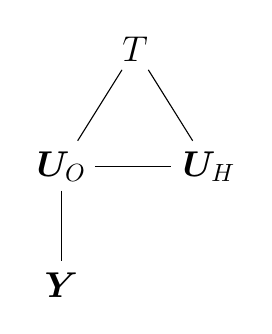
\begin{tikzpicture}	
      \tikzstyle{every edge}=[-,>=stealth',shorten >=1pt,auto,thin,draw]
		\node[observed] (A1) at (0.625*\edgeunit, 2*\edgeunit) {$T$};
		\node[observed] (A2) at (0*\edgeunit, 1*\edgeunit) {$\Ubf_O$};
		\node[observed] (A3) at (1.25*\edgeunit, 1*\edgeunit) {$\Ubf_H$};
		\node[observed] (A4) at (0*\edgeunit, 0*\edgeunit) {$\Ybf$};
		\path (A1) edge [] (A2)
        (A1) edge [] (A3)
        (A2) edge [] (A3)
        (A2) edge [] (A4);
	\end{tikzpicture}
\end{center}

\subsection{Distributions}
\label{distrib}
 
The complete vector of underlying parameters $\Ubf$ follows a mixture of normalized Gaussian distributions on the space of all existing spanning trees.
\begin{align*}
(\Ubf_O,\Ubf_H) &\sim \sum_{T \in \mathcal{T}} p(T) \mathcal{N}(0,R_T) \\
\end{align*}

 
Conditionally on the dependency structure $T$, $\Ubf$ is a centered Gaussian variable, with covariance matrix $R_T$ defined by block. As latent vectors are normalized, $R_T$ is a correlation matrix, and we define $\Omega$ its inverse. We obtain the following distributions:
\begin{align*}
(\Ubf_O,\Ubf_H)|T & \sim\mathcal{N}(0,R_T)\\
\end{align*}
 
 

\subsection{Assumptions}
\paragraph{Assumption A:} The missing latent variables are not connected with each other. The $H$ bloc of $\Omega_T$ should thus be diagonal.
 
 
 \section{Variational EM inference}
\subsection{Approximation of the likelihood}
\paragraph{Joint likelihood:}
The graphical model gives the following writing of the joint likelihood:
\begin{align*}
p(\Ybf,\Ubf,T)& = p(T) \: p(\Ubf|T) \: p(\Ybf|\Ubf) \\
&= p(T)\: p(\Ubf_O,\Ubf_H|T) \: p(\Ybf|\Ubf_O,\Ubf_H) \\
&= p(T) \: p(\Ubf_O|T) \: p(\Ubf_H | \Ubf_O,T)  \: p(\Ybf|\Ubf_O)
\end{align*} 


\paragraph{Variational approximation:}

Here $p(T,\Ubf \mid \Ybf)$ is untractable. We adopt a variational approximation aiming to maximise a lower bound of the log-likelihood of observed data $\log p(\Ybf)$, namely  
\begin{align*}
    \mathcal{J}(\Ybf; g,h)
    & = \log p(\Ybf) - KL\left[q(T,\Ubf) \mid\mid p(T,\Ubf \mid \Ybf)\right]
\end{align*}
Where KL is the Küllback-Leibler divergence. The approximation we adopt relies on factorizing $q$ in the product of two distributions $h$ and $g$ relating respectively to $\Ubf$  and $T$: 
$$p(T,\Ubf \mid\Ybf) \approx  q(\Ubf,T) = g(T)\:h(\Ubf).$$

 A consequence of this hypothesis is the contributions of   $\Esp_h[\log p(\Ubf\mid T)]$ and $\log p(T)$ --~only terms involving $T$ in the lower bound~-- writing as sums on the edges. As distribution   $g$ minimizes the KL divergence, it has to factorizes on the edges as well and hence:
$ g(T) = \left(\prod_{kl} \widetilde{\beta}_{Tkl} \right) / \widetilde{B}_T$. \\

Moreover, it follows from the independence of the samples that $h$ is a product law: $ h(\Ubf) = \prod_i h_i(\Ubf_i)$. Our variational approximation consists in assuming that each of its components is a multivariate Gaussian: $h(\Ubf_i) = \Ncal(\Ubf_i; \mbf_i, \Sbf_i)$, where $\Sbf_i$ is diagonal, meaning that $\Ubf_H$ and $\Ubf_O$ are independent under distribution $h$.  In the following we use the  $n\times (p+r)$ matrices $M$ and $S$ which compile respectively all vectors of means $\mbf_i$ and diagonals of variances $\Sbf_i$.


\paragraph{Lower bound:}
The lower bound of our model writes:
\begin{align*}
\mathcal{J}(\Ybf; g,h)&=\log p(\Ybf) - KL\left[g(T) h(\Ubf) \middle\vert\middle\vert\ p(T,\Ubf | \Ybf)\right]\\
&= \log p(\Ybf) - \Esp_{gh}[\log( g(T) h(\Ubf)) - \log p(\Ubf,T\mid \Ybf) ]\\
&= \log p(\Ybf) - \Esp_{gh}[\log g(T) + \log h(\Ubf) ] + \Esp_{gh}[\log p(\Ybf,\Ubf,T)] - \Esp_{gh}[\log p(\Ybf)]\\
&= \Esp_{gh} [\log p(\Ybf,\Ubf,T)] + \entr[g(T)] + \entr[h(\Zbf)]
\end{align*}

\begin{equation}
\label{firstJ}
 \boxed{\mathcal{J}(\Ybf; g,h) = \Esp_{gh} \Big[\log \big(p_\beta(T)\:p_{\Omega_T}(\Ubf\mid T)\:p_{\theta, \sigma}(\Ybf\mid \Ubf)\big)\Big] + \entr[g_{\widetilde{\beta}_T}(T)] + \entr[h_{M,S}(\Ubf)]}
\end{equation}
Thus the model's parameters are $\Phi = (\theta,\sigma,M,S,\widetilde{\beta}_T, \beta,  \Omega_T)$.

\subsection{PLNmodels: optimizing in $\theta$, $\sigma$, and $h(\Ubf_O)$:}
\citet{CMR18} compute the lower bound of a VEM for the original PLN model, that is where no missing actor is assumed and the independence structure of the latent layer of parameters is not supposed to be faithful to a tree: $p(\Ubf_O) = \mathcal{N}(0,R)$. We let $\mathcal{J}_{PLN}$ denote this lower bound, which writes:
$$\mathcal{J}_{PLN} = \Esp_h[\log p(\Ubf_O)] + \Esp_h[\log p(\Ybf|\Ubf_O)] + \entr[h(\Ubf_O)].$$ $\mathcal{J}_{PLN}$ is implemented  in the R package \texttt{PLNmodels}, and can be used in our computation as well.

\subsubsection{Rewriting  $\mathcal{J}(\Ybf; g,h)$}
Let's first separate observed and unobserved latent variables:
\begin{align*}
\mathcal{J}(\Ybf; g,h)&= \Esp_{gh}\Big[\log \big(p(T)\:  p(\Ubf_H| \Ubf_O,T)\: p(\Ubf_O|T)\:p(\Ybf|\Ubf_O)\big)\Big] + \entr[g(T)] +\entr[h(\Ubf_H,\Ubf_O)]
\end{align*}

 $\Ubf_O$ and $\Ubf_H$ being independent under the $h$ distribution, we have that $\entr[h(\Ubf_H,\Ubf_O)] =\entr[h(\Ubf_O)] +\entr[h(\Ubf_H)]$. Now using the hypothesis of independence of $g$ and $h$, we obtain quantities with separate dependencies:
\begin{align}
\mathcal{J}(\Ybf; g,h)&=  \Esp_{gh}[\log p(\Ubf_O | T)] +\Esp_h[\log p(\Ybf|\Ubf_O)]+\entr[h(\Ubf_O)]  \label{PLNlike}\\
& \;\; + \Esp_{gh}[\log p(\Ubf_H | \Ubf_O,T) ]+\Esp_g[\log p(T)] +\entr[g(T)]+\entr[h(\Ubf_H)] \label{new}
\end{align}

Which we write as below, where each term of the right hand-side corresponds to each line above:
$$\mathcal{J}(\Ybf; g,h)= \Esp_g[\mathcal{J}_{\Ubf_O}(\Ybf;h)] + \mathcal{J}_{\Ubf_H|\Ubf_O}(\Ybf;h,g)]$$
The idea is to take advantage of the maximization of  $\mathcal{J}_{PLN}$, which appears as follows in $\Esp_g[\mathcal{J}_{\Ubf_O}(\Ybf;h)] $:
\begin{align*}
\mathcal{J}_{\Ubf_O}(\Ybf;h) &= \Esp_h[\log p(\Ubf_O|T)] + \Esp_h[\log p(\Ybf|\Ubf_O)]+\entr[h(\Ubf_O)]\\
&= \mathcal{J}_{PLN} + \big(\Esp_h[\log p(\Ubf_O|T)-\log p(\Ubf_O) ]\big)\\
\Esp_g[\mathcal{J}_{\Ubf_O}(\Ybf;h)] &= \mathcal{J}_{PLN} + \Big(\Esp_h\big[\Esp_g[\log p(\Ubf_O|T)]-\log p(\Ubf_O) \big]\Big)
\end{align*}
Noticing that $\log p(\Ubf_O) = \log (\Esp_g[ \log p(\Ubf_O|T)])$, the last term above is negative according to Jensen's inequality.

 \subsubsection{Maximization of $\mathcal{J}(\Ybf; g,h)$}

$$\argmax_{\theta}\Big\{\mathcal{J}(\Ybf; g,h)\Big\} = \argmax_{\theta}\Big\{\mathcal{J}_{PLN}\Big\} $$
$$ (\tilde{M}_O, \tilde{S}_O) = \argmax_{M_O,S_O}\Big\{\mathcal{J}_{PLN}\Big\} $$

\subsection{VE step: optimizing in $g$ and $h(\Zbf_H)$}
The VE step minimizes the Küllback-Leibler divergence between the approximated and the aimed distributions :

$$  \argmin_{g,h(\Ubf_H)} KL\left(g(T)h(\Ubf) \mid\mid p(\Ubf,T|\Ybf)\right)$$

\begin{align*}
KL\left(g(T)h(\Ubf) \mid\mid  p(\Ubf,T|\Ybf)\right) &= \Esp_{gh}\left[\log g(T)h(\Ubf) - \log p(\Ubf,T\mid \Ybf) \right]\\
&= \Esp_{gh}\left[\log g(T)h(\Ubf) - \log p(\Ybf,\Ubf,T) + \log p(\Ybf)  \right]\\
&= \Esp_{gh}\left[\log g(T)+ \log h(\Ubf) - \log (p(T)p(\Ubf\mid T) p(\Ybf\mid \Ubf_O)) + \log p(\Ybf)  \right]\\
&= -\Esp_{gh}[\log p(\Ubf \mid T) ] - \Esp_g[\log p(T) - \log g(T)] - \entr[h(\Ubf)]\\
& \;\;\;\; -\Esp_h[\log p(\Ybf \mid \Ubf_O)] +\log p(\Ybf) 
\end{align*}
Distributions $p(\Ybf)$ and $p(\Ybf\mid \Ubf_O)$  do not depend on distributions $g$ and $h(\Ubf_H)$. Moreover, as $\Ubf_O$ and $\Ubf_H$ are independant under the $h$ distribution, $\entr[h(\Ubf)] = \entr[h(\Ubf_O)]+ \entr[h(\Ubf_H)]$ and  $\entr[h(\Ubf_O)]$ is already optimized. We obtain:
 
\begin{empheq}[box=\widefbox]{align*}
\argmin_{g,h(\Ubf_H)} KL  &=\argmin_{g,h(\Ubf_H)} \Big\{ -\Esp_{gh}[\log p(\Ubf \mid T) ] - \Esp_g[\log p(T) - \log g(T)] -\entr[h(\Ubf_H)] \Big\}
\end{empheq}
 
 During the minimization, we will use the optimized distribution $h(\Ubf_O)^* = \prod_i^n \mathcal{N}(\widetilde{\mbf}_{Oi}, \widetilde{S}_{Oi})$, its parameters being gathered in $n\times p$ matrices $\widetilde{M}_O$ and $\widetilde{S}_O$.
 
 \subsubsection{Details of  $\Esp_{gh}[\log p(\Ubf \mid T) ]$} 
 $$\log p(\Ubf \mid T) = -\frac{n}{2} \log |R_T| - \frac{1}{2} Tr(\Omega_T \times \Ubf^\intercal \Ubf) $$
 Taking the expectation, and by independence of $g$ and $h$:
 $$\Esp_{gh} [\log p(\Ubf \mid T)] = \frac{n}{2} \Esp_{gh} [\log | \Omega_T|] - \frac{1}{2} Tr(\Esp_g[\Omega_T] \Esp_h[\boldsymbol{U}^\intercal \boldsymbol{U}])$$
 
 We let $SSD$ denote the sum of squared deviance. From the definition of the $h$ distribution: $$ \Esp_h[\Ubf^\intercal \Ubf] = M^\intercal M + S = SSD$$
  $SSD$ is a sufficient statistic of the distribution, and  as latent vectors have variance 1, $SSD/n$ has diagonal 1.
 
\paragraph{Expectation of the log-determinant of $\Omega_T$\\}
Thanks to $\Omega_T$ being tree-structured, its determinant factorizes on the edges of $T$ as follows:
\begin{align*}
|\Omega_T| &=\frac{\prod_k |R_{Tkk}|^{deg(k)-1}}{\prod_{kl \in T} |R_{Tkl}|} =  \Big(\prod_{kl \in T} (1-\rho_{Tkl}^2)\Big)^{-1},
 \end{align*}

 This gives $$ \Esp_g[\log|\Omega_T|]=-\frac{1}{2}\sum_{kl} \Esp_g[ I_{Tkl}\log(1-\rho_{Tkl}^2)].$$
\paragraph{Trace of expectations\\}
 
\begin{align*}
Tr(\Esp_g[\Omega_T] SSD) &= \sum_{kl} \Esp_g[I_{Tkl} \omega_{Tkl}ssd_{kl}] + \sum_k \Esp_g[\omega_{Tkk} ssd_{kk}] 
\end{align*}

Finally, 
\begin{empheq}[box=\lesswidefbox]{align*}
\Esp_{gh} [\log p(\Ubf \mid T)] =-  \frac{n}{4}\sum _{k \neq l} \Esp_g\Big[ I_{Tkl}\Big(\log(1-\rho_{Tkl}^2)+ \omega_{Tkl} \frac{ssd_{kl}}{n}\Big)\Big] -\frac{1}{2}  \sum_k \Esp_g[\omega_{Tkk} ssd_{kk}] 
 \end{empheq}
 If we can provide estimates $\hat{\rho}_{kl}$ and $\widehat{\Omega}=(\hat{\omega}_{kl})_{kl}$ that are independent of $T$, then using that $SSD$ has diagonal $n$ the above expectation can be estimated as
 $$\Esp_{gh} [\log p(\Ubf \mid T)] =-  \frac{n}{4}\sum _{k \neq l} P_{kl}\Big(\log(1-\hat{\rho}_{kl}^2)+ \hat{\omega}_{kl} \frac{ssd_{kl}}{n}\Big) -\frac{n}{2} \sum_{k} \hat{\omega}_{kk}$$
\subsubsection{Details of $\Esp_g[\log g(T) - \log p(T)]$}
\begin{align*}
\log g(T) - \log p(T) &= \left(  \sum_{j<k}I_{Tkl}\log \widetilde{\beta}_{Tjk} - \log \widetilde{B}_T\right) - \left(  \sum_{j<k} I_{Tkl}\log {\beta}_{jk} - \log {B}\right)\\
&=\frac{1}{2}\sum_{jk} I_{Tkl}\log \frac{\widetilde{\beta}_{Tjk}}{{\beta}_{jk}} - \log \frac{\widetilde{B}_T}{B}
\end{align*}
$$\boxed{
\Esp_g[\log g(T) - \log p(T)] = \frac{1}{2}\sum_{jk} \Esp_g\Big[I_{Tkl} \big(\log \widetilde{\beta}_{Tjk}-\log(\beta_{jk})\big)\Big] - \log \frac{\Esp_g[\widetilde{B}_T]}{B} }$$
If we can provide estimates $\widetilde{\beta}_{kl}$ that do not depend on $T$, the above expectation can be estimated as:
$$ \Esp_g[\log g(T) - \log p(T)] = \frac{1}{2}\sum_{jk} P_{kl} \big(\log \widetilde{\beta}_{jk}-\log(\beta_{jk})\big) - \log \frac{\widetilde{B}}{B} $$
 \subsubsection{Details of $\entr[h(\Ubf_H)]$}
 
 The entropy of the Gaussian multivariate vector $\Ubf_H$ mainly depends on its variance matrix $S_H$. By definition of $S_H$ we have:
 \begin{align*}
 \log |S_H| &= \log(\prod_{k=p+1}^{p+r} \sum_{i=1}^n S_{ik})
\end{align*}
which gives the following entropy:
\begin{align*}
\entr[h(\Ubf_H)]&= \frac{1}{2} \log |S_H| + \frac{nr}{2}(1+\log(2\pi))\\
 &=\frac{1}{2}\left[ \sum_{k=p+1}^{p+r} \log\left(\sum_{i=1}^n S_{ik}\right)+ nr(1+\log 2\pi )\right]
\end{align*}

\subsubsection{Final quantity to optimize:}
\begin{align*}
\argmin_{g,h(\Ubf_H)} KL  &=\argmin_{g,h(\Ubf_H)}  \Big\{-\Esp_{gh}[\log p(\Ubf \mid T) ] + \Esp_g[\log g(T) - \log p(T)-\entr[h(\Ubf_H)]\Big\}\\
&= \argmin_{g,h(\Ubf_H)}  \bigg\{   \frac{n}{2}\sum _{k \neq l} \Esp_g\Big[ I_{Tkl}\Big(\frac{1}{2}\log(1-\rho_{Tkl}^2)+ \omega_{Tkl} \frac{ssd_{kl}}{n}\Big)\Big] +\frac{1}{2}  \sum_k \Esp_g[\omega_{Tkk} ssd_{kk}] \\
& \;\;\;\; +\frac{1}{2}\sum_{jk} \Esp_g\Big[I_{Tkl} \big(\log \widetilde{\beta}_{Tjk}-\log(\beta_{jk})\big)\Big] - \log \frac{\Esp_g[\widetilde{B}_T]}{B} -\frac{1}{2}\sum_{k\in H} \log\left(\sum_i \widetilde{S}_{ik}\right) \bigg\}
\end{align*}
With estimates independent of $T$:
\begin{align*}
\argmin_{g,h(\Ubf_H)} KL  &=\argmin_{g,h(\Ubf_H)}  \Big\{-\Esp_{gh}[\log p(\Ubf \mid T) ] + \Esp_g[\log g(T) - \log p(T)-\entr[h(\Ubf_H)]\Big\}\\
&= \argmin_{g,h(\Ubf_H)}  \bigg\{ \frac{n}{2}\Big(\sum _{ k \neq l} P_{kl}\Big(\frac{1}{2} \log (1-\rho_{kl}^2) + \omega_{kl} \frac{ssd_{kl}}{n}\Big) +  \sum_{k} \omega_{kk} \Big)\\
& \;\;\;\; + \frac{1}{2}\sum_{ k\neq l}P_{kl} \left(\log \frac{\widetilde{\beta}_{kl}}{{\beta}_{kl}}\right) - \log \frac{\widetilde{B}}{B} -\frac{1}{2}\sum_{k\in H} \log\left(\sum_i \widetilde{S}_{ik}\right) \bigg\}
\end{align*}
 
 
 \subsubsection{Update formulas for $\widetilde{\beta}$ and $M_H$ }

\paragraph{Edges weights under the $g$ distribution \\}
Let's isolate the terms referring to the edges in the expression to be minimized:
$$ \frac{1}{2}\sum _{k \neq l} \Esp_g\Big[I_{Tkl}\Big(\frac{n}{2} \log(1-\rho_{Tkl}^2)+ \omega_{Tkl}ssd_{kl}+\log \widetilde{\beta}_{Tjk}-\log\beta_{jk}\Big)\Big]  $$
 
 
As $g$ is a discrete distribution on the space of spanning trees, maximizing an expectation taken on $g$ is equivalent to maximizing each expression inside the expectation on each tree. In the above sum, equating what is inside the expectation in $g$ of the term $kl$ to zero, we obtain:
 $$\log \widetilde{\beta}_{Tkl} = \log \beta_{kl} - \frac{n}{2} \log  (1-\rho_{Tkl}^2) - \omega_{Tkl}\:ssd_{kl}$$
 
Which gives the following update formula for $\widetilde{\beta}_{Tkl}$:
 
  $$\boxed{\displaystyle \widetilde{\beta}_{Tkl} = \beta_{kl} \: (1-\rho_{Tkl}^2)^{-n/2} \exp( -\omega_{Tkl}\: ssd_{kl} ) }$$


\paragraph{Means of the hidden part of the latent Gaussian vector under the $h$ distribution \\}
Means $M_H$ only appear in the $H$, $OH$ and $HO$ blocs of $SSD$. Denoting $\bar{\Omega} = (\bar{\omega}_{kl})_{kl} =\Esp_g[\Omega_T]$, the derivative of KL with respect to mean $M_{jh}$ for the $j^\text{th}$ sample of species $h\in H$ writes:

\begin{align*}
\frac{\partial KL}{\partial M_{jh}} &= \frac{\partial}{\partial M_{jh}}\Big(2\sum_{ (k, l) \in H\times O}\bar{\omega}_{kl} (M^\intercal M)_{kl} + \sum_{k\in H} \bar{\omega}_{kk} (M^\intercal M)_{kk}\Big)\\
&=\frac{\partial}{\partial M_{jh}}\Big(2\sum_i \Big(\sum_{k\in H} M_{ik}\sum_{l\in O}\bar{\omega}_{kl} M_{il}\Big) + \sum_{k\in H} (\bar{\omega}_{kk} \sum_i M_{ik}^2)\Big)\\
&=   \sum_{l \in O } M_{jl} \bar{\omega}_{hl} + M_{jh} \bar{\omega}_{hh}
\end{align*}
\begin{align*}
\frac{\partial KL}{\partial M_{jh}}  = 0\iff M_{jh} &= -\frac{1}{\bar{\omega}_{hh}} \sum_{l\in O} M_{jl}\bar{\omega}_{lh}\\
&=-\frac{M_{jO} \bar{\Omega}_{Oh}}{\bar{\omega}_{hh}}
\end{align*}

As $\bar{\Omega}_H$ is diagonal following assumption A, this  matricially comes down to
$$\boxed{ M_H = -M_O\bar{\Omega}_{OH} \bar{\Omega}_H^{-1}}$$


\paragraph{Variances of the hidden part of the latent Gaussian vector under the $h$ distribution \\}
$S_H$ is updated following the constraint that $SSD$ has to be of diagonal $n$. By definition, for $h\in H$ we have that $S_H = \sum_i s_{ih}$, therefore the constraint on the diagonal of $SSD$ does not allow to identify each of the $s_{ih}$, which we thus consider all equal, and we define $s_h$ such that for all $ h\in H$ and all $ i\in \{1,...,n\}$, $s_{ih} = s_h$.  By definition, the diagonal term $hh$ of $SSD$ is as follows:

\begin{align*}
& M_h^\intercal M_h+ n\:s_h = n\\
\iff &\boxed{s_h = 1-\frac{ M_h^\intercal M_h}{n}}
\end{align*}

\subsubsection{Computing edge probabilities under $g$}
During computations, we need the edge probability under the $g$ distribution. This can be computed as the sum of probabilities of trees containing this edge:

\begin{align*}
\mathds{P}_g(kl \in T)  &= \sum_{\substack{T  \in \mathcal{T} \\ kl \in T }} g(T) =\frac{1}{\widetilde{B}} \sum_{\substack{T  \in \mathcal{T} \\ kl \in T }} \prod_{uv \in T} \widetilde{\beta}_{uv}
\end{align*}
where $\displaystyle \widetilde{B}= \sum_{T \in \mathcal{T} }\prod_{uv \in T}  \widetilde{\beta}_{uv}$.\\

 This is again a sum-product form, but on a special set of trees. This can be efficiently computed using a formula from \citet{kirshner} (Theorem 3), stated in the appendix.
 
 
 \subsection{M step: optimizing in $(\beta, \Omega_T)$}
 The M step aims at maximizing the lower bound in the parameters referring to original distributions for $T$ and $\Ubf|T$, therefore $\beta$ and $\Omega_T$. From Eq.(\ref{firstJ}) we obtain that: 
$$ \argmax_{\beta, \Omega} \mathcal{J}(\Ybf ; g,h) =\argmax_{\beta, \Omega} \left\{ \Esp_{gh} [\log (p_\beta(T)p_{\Omega_T}(\Ubf\mid T) ]\right\} $$

As distributions of VE step mimic original ones, computations are very similar. We get:
\begin{align*}
\log (p_\beta(T)p_{\Omega_T}(\Ubf\mid T))  &= \frac{1}{2}\sum_{kl} I_{Tkl} \log \beta_{kl} - \log B + \frac{n}{2}\log |\Omega_T| - \frac{1}{2}Tr(\Omega_T \Ubf^\intercal \Ubf)\\
\Esp_{gh} [\log (p_\beta(T)p_{\Omega_T}(\Ubf\mid T) ] &= \frac{1}{2}\sum_{kl} P_{kl} \log\beta_{kl} +\frac{n}{2} \Esp_g[\log |\Omega_T|] -\frac{1}{2} Tr(\bar{\Omega} \; SSD)- \log B
\end{align*}

Reminding that $ \Esp_g[\log|\Omega_T|]=-\frac{1}{2}\sum_{kl} \Esp_g[ I_{Tkl}\log(1-\rho_{Tkl}^2)]$,  we obtain:
\begin{align*}
\Esp_{gh} [\log (p_\beta(T)p_{\Omega_T}(\Ubf\mid T) ] &=\frac{1}{2}\sum_{kl} P_{kl} \log  \beta_{kl} - \log B - \frac{n}{4} \sum_{kl} \Esp_g[ I_{Tkl}\log(1-\rho_{Tkl}^2)]  - \frac{1}{2}Tr\big(\bar{\Omega}\: SSD\big) 
\end{align*}
 
 \subsubsection{Update formula for $\beta$}
 The derivative of $ \mathcal{J}(\Ybf ; g,h)$ with respect to weight $\beta_{kl}$ of edge $kl$ is:
 
 \begin{align*}
\frac{\partial}{\partial_{\beta_{kl}}} \mathcal{J}(\Ybf ; g,h) &=  \frac{\partial}{\partial_{\beta_{kl}}} \Esp_{gh} [\log (p_\beta(T)p_{\Omega_T}(\Ubf\mid T) ] \\
&= \frac{P_{kl}}{\beta_{kl}} - \frac{\partial_{\beta_{kl}} B }{B} \\
\end{align*}

The derivative of the normalization constant with respect to $\beta_{kl}$ is the derivative of an output from the Matrix Tree theorem with respect to one of the weight's matrix entry. This quantity is given by \citet{Meila} (Lemma 2). Defining matrix $Q(\betabf)$ as showed in the appendix, then $\partial_{\beta_{kl}} B = B\times Q(\betabf)_{kl}$ and:
$$\frac{\partial}{\partial_{\beta_{kl}}} \mathcal{J}(\Ybf ; g,h) 
=0 \iff  \boxed{\widehat{\beta}_{kl} = \frac{P_{kl}}{ Q(\betabf)_{kl}} }$$

 \subsubsection{Update formula for $\Omega_T$ and $R$}
 \paragraph{Notations\\}
In what follows, for any $q\times q$  matrix $A$, $A_{kl}$ will refer to the bloc $kl$ of $A$: $A_{kl}=(a_{ij})_{\{i,j\}\in\{k,l\}}$.   $[A_{kl}]^q$ will then denote the matrix obtained by filling up with zero entries to obtain full dimension $q\times q$, so that:
$$([A_{kl}]^q )_{ij}=\left\{ \begin{array}{rl}
a_{ij} & \text{if } \{i,j\}\in\{k,l\}\\
0 &  \text{if } \{i,j\}\in\{1,..., q\}_{\setminus kl}
\end{array}\right.$$

 
\paragraph{Justification\\}

As $g$ is a discrete distribution on the space of spanning trees, maximizing an expectation in $g$ is equivalent to maximizing the expression for each tree. Thus,
$$ \max\big(\Esp_g[\mathcal{J}_T(\Ybf;h)]\big) = \Esp_g\big[\max(\mathcal{J}_T(\Ybf;h))\big]$$
and as soon as a maximum likelihood estimator exists for a parameter of $\mathcal{J}_T(\Ybf;h)$, using it will maximize $\mathcal{J}(\Ybf;h,g)$ as well. 

\paragraph{Computation\\}
 We use the maximum likelihood estimates $\hat{\rho}$ and $\hat{\Omega}_T$ established in \citet{Lau96}, which depends only on the $SSD$ matrix and the underlying dependency structure.
  The correlation corresponding to an existing edge in the structure $T$ is estimated using
  $$ \forall kl\in T,\boxed{\hat{\rho}_{kl} = ssd_{kl}/n}.$$
  Note that this maximum likelihood estimator do not depend on $T$.\\
  
   The estimator  $\hat{\Omega}_T$  writes as the following in our context:
\begin{align*}
\widehat{\Omega}_T &= n  \sum_{kl\in T}   [(SSD_{kl})^{-1}]^{p+r} - n\sum_k (deg(k)-1)[(SSD_{kk})^{-1}]^{p+r}\\
&=n \sum_{kl\in T}  [(SSD_{kl})^{-1} - (SSD_{kk})^{-1} -  (SSD_{ll})^{-1} ]^{p+r} + n\sum_k[(SSD_{kk})^{-1}]^{p+r}
\end{align*}
As SSD has diagonal n, the expression simplifies. Denoting $I_d$ the identity matrix of dimension $d$ we obtain:
$$\widehat{\Omega}_T =n\sum_{kl\in T} [(SSD_{kl})^{-1} -\frac{1}{n} I_2]^{p+r}+ I_{p+r}$$

We can detail each bloc matrices as follows:
\[
n\times [(SSD_{kl})^{-1} - \frac{1}{n}I_2] = \frac{1}{1-(ssd_{kl}/n)^2}
\left(\begin{array}{cc}
		(ssd_{kl}/n)^2   & -ssd_{kl}/n\\
		-ssd_{kl}/n& (ssd_{kl}/n)^2 
		\end{array}\right)
\]
This allows to write the following:
 \[ \boxed{\widehat{\Omega}_{Tkl}=\left\{\begin{array}{cl}I_{Tkl}
  \times\dfrac{ -ssd_{kl}/n}{1-(ssd_{kl}/n)^2} & ,k\neq l\\\\
 \sum_l I_{Tkl} \dfrac{(ssd_{kl}/n)^2}{1-(ssd_{kl}/n)^2} +1 & ,k=l
 \end{array}\right.
 }\]
It shows here that using only trees comes down to only manipulate inverses of $2\times 2$ matrices, and yields values of non-nul off-diagonal terms of $\hat{\Omega}_T$ that are independent of $T$. This means that the common non-nul off-diagonal terms of precision matrices of different trees will be equal. \\

 Note that on the other hand, the diagonal depends on $T$ and its $k$ term depends on the degree of node $k$ as follows:

$$\widehat{\Omega}_{Tkk} =\sum_l \frac{I_{Tkl} }{1-(ssd_{kl}/n)^2} -(deg(k)-1).$$
 
Let's now consider the expectation in $g$:

$$\Esp_g[\widehat{\Omega}_T]= \widehat{\bar{\Omega}}= n\sum_{kl} P_{kl} \had [(SSD_{kl})^{-1} - I_2]^{p+r} + I_{p+r}$$
 The expectation above defines a matrix which off-diagonal term $kl$ and diagonal term $kk$ write as follows:
$$\widehat{\bar{\Omega}}_{kl} = P_{kl} \left(\frac{-ssd_{kl}/n}{1-(ssd_{kl}/n)^2} \right)\text{\hspace{0.5cm},\hspace{1cm}}\widehat{\bar{\Omega}}_{kk} = \sum_l P_{kl} \frac{(ssd_{kl}/n)^2}{1-(ssd_{kl}/n)^2} +1 $$
 
 
%%%%%%%%%%%%%% 
\newpage
\bibliographystyle{apsrev} %tested plainnat
\bibliography{bibi}
 \appendix
 \section{Algebraic Tools}
 For any matrix $\Wbf$, we denote its entry in row $u$ and column $v$ by $[\Wbf]_{uv}$. We define the Laplacian matrix $\Qbf$ of a symmetric matrix $\Wbf=[w_{jk} ]_{1\leq j,k\leq p}$ as follows :
 
\[
 [\Qbf]_{jk}  =\begin{cases}
    -w_{jk}  & 1\leq j<k \leq p\\
    \sum_{u=1}^p w_{ju} & 1\leq j=k \leq p.
    \end{cases}
\]
 
We further denote $\Wbf^{uv}$ the matrix $\Wbf$ deprived from its $u$th row and $v$th column and we remind that the $(u, v)$-minor of $\Wbf$ is the determinant of this deprived matrix, that is $|\Wbf^{uv}|$.

\begin{theorem}[Matrix Tree Theorem  \cite{matrixtree,Meila}] \label{thm:MTT}
    For any symmetric weight matrix W, the sum over all spanning trees of the product of the weights of their edges is equal to any minor of its Laplacian. That is, for any $1 \leq u, v \leq p$,
 
   \[
    W := \sum_{T\in\mathcal{T}} \prod_{(j, k)\in T} w_{jk} = |\Qbf^{uv}|.
    \]
   
\end{theorem}    

In the following, without loss of generality, we will choose $\Qbf^{pp}$. As an extension of this result, \cite{Meila} provide a close form expression for the derivative of $W$ with respect to each entry of $\Wbf$. 

\begin{lemma} [\cite{Meila}] \label{lem:Meila}
    Define the entries of the symmetric matrix $\Mbf$ as
 
\[    
 [\Mbf]_{jk} =\begin{cases}
    \left[(\Qbf^{pp})^{-1}\right]_{jj} + \left[(\Qbf^{pp})^{-1}\right]_{kk} -2\left[(\Qbf^{pp})^{-1}\right]_{jk} & 1\leq j<k < p\\
    \left[(\Qbf^{pp})^{-1}\right]_{jj} & k=p, 1\leq j \leq p  \\
    0 & 1\leq j=k \leq p.
    \end{cases}
\]
 
it holds that
 
$$
\partial_{w_{jk}} W = [\Mbf]_{jk}  \times W.
$$
\end{lemma}
\begin{lemma} [\cite{kirshner}] \label{lem:Kirshner}
    Let $p_W$ be a distribution on the space of spanning trees, such that $p_W(T)=\prod_{kl\in T} w_{kl} / W$, where $W$ is defined as in Theorem \ref{thm:MTT}. Taking the symmetric matrix $\Mbf$ as defined in Lemma  \ref{lem:Meila}, the probability for an edge $kl$ to be in the tree $T$ writes:
 
$$\mathds{P}\{kl\in T\} = \sum_{T\in \mathcal{T}} p_W(T)= w_{kl}\: \Mbf_{kl}$$
\end{lemma}
 \section{Divers}
 
\subsection{Dérivation du log-déterminant}
On peut dériver par rapport à $\Omega$, en supposant la première ligne :
\begin{align}
    \partial_{\Omega}\left(\Esp_{gh}\left[\log p(\Zbf | T)\right] \right)&=  \Esp_{gh}\left[\partial_{\Omega}( \log p(\Zbf | T) )\right] \\
    &=\Esp_{gh}\left[\frac{n}{2}\partial_{\Omega}( \log |\Omega_T|) -\frac{1}{2} \partial_\Omega (Tr(\Omega_T \; \Zbf^\intercal \Zbf ))\right]
\end{align}

\paragraph{\underline{$\partial_{\Omega}( \log |\Omega_T|)$} :}
 $$\log |I_T \cdot \Omega| = \log \big(\sum_{k=1}^q (I_T\cdot \Omega)_{ik} \mathsf{Com}_{ik}\big)$$
Le terme $\omega_{ik}$ n'apparaît pas dans le cofacteur $\mathsf{Com}_{ik}$, ce qui donne :
\begin{align*}
    \partial_{\omega_{ij}} \log |I_T\cdot \Omega| &= (I_T)_{ij} \frac{\mathsf{Com}_{ij}}{|I_T\cdot \Omega |}
\end{align*}
Or on a $(I_T\cdot \Omega)^{-1} = \frac{1}{|I_T \cdot \Omega|}\times \mathsf{Com}^\intercal$, et en particulier par symétrie de $\Omega_T$ on a que $(I_T\cdot \Omega)_{ij}^{-1}=\frac{\mathsf{Com}_{ij}}{|I_T\cdot \Omega |}$.

Donc 
\begin{align}
         &\partial_{\omega_{ij}} \log |I_T\cdot \Omega| = (I_T)_{ij} (I_T\Omega)_{ij}^{-1}
\end{align}
Par symétrie :
\begin{align}
    &\partial_\Omega \log |I_T\cdot \Omega| = 2I_T \cdot \Omega_T^{-1}\\\\
    \iff &\Esp_g \big( \partial_\Omega \log |\Omega_T| \big) = 2\Esp_g (I_T\cdot \Sigma_T) 
\end{align}

\paragraph{\underline{$ \partial_\Omega (Tr(\Omega_T \; Q ))$}:}
\begin{align}
    \partial_\Omega \Esp_{gh}[Tr(\Omega_T \Zbf^\intercal \Zbf)]&=\partial_\Omega Tr(\Esp_g[\Omega_T]Q)\\
    &=\partial_\Omega Tr((P\cdot\Omega)Q)\\
    &=2P\cdot Q
\end{align}
D'où $$ \Esp_g (I_T\cdot \Sigma_T)  = \frac{PQ}{n}$$

Et également 
$$\boxed{n I_T\cdot \hat{\Sigma}_T = I_T\cdot \Esp_h[\Zbf^\intercal \Zbf] = I_T\cdot \widehat{SSD}}$$
\subsection{Calcul du déterminant}
Soit $R=(\rho_{ij})_{ij}$ une matrice de corrélations, et $R^{-1}= \Omega$. D'après Lauritzen (5.12):
$$\frac{\omega_{\mu\gamma}^2}{\omega_{\mu\mu}\omega_{\gamma\gamma}} = c_{\mu\gamma}^2 = 1-\frac{|R|\;|R_{\setminus \{\mu\gamma\}}|}{|R_{\setminus\gamma}|\;|R_{\setminus \mu}|} $$
Si R est fidèle à un graphe $\mathcal{G}$ décomposable, alors son déterminant dépend des déterminants des blocs de $R$ défini par les cliques et les séparateurs du graphe, tel que :
$$|R| = \frac{\prod_{C \in \mathcal{C}} |R_C|}{\prod_{S \in \mathcal{S}} |R_S|^{\nu(S)}} $$
où $\nu(S)$ est la multiplicité du séparateur $S$. En particulier si $\mathcal{G}$ est un arbre $T$, les cliques sont les arêtes et les séparateurs les noeuds. Comme $R$ est de diagonale 1, son déterminant s'obtient simplement :
\begin{align*}
    |R| &=  \prod_{kl\in T} (1-\rho_{kl}^2)\\
\end{align*}
Lorsqu'un noeud $\gamma$ est retiré de $T$, $R_{\setminus \gamma}$ devient fidèle à un graphe marginalisé sur $\gamma$, où apparaît une clique $C_\gamma$ formée par l'ensemble des anciens voisins de $\gamma$, et le reste du graphe reste inchangé. L'ensemble des cliques du graphe marginalisé est donc constitué de $C_\gamma$, et des arêtes dont aucune extrémité n'est $\gamma$ dans $T$.
\begin{figure}[h]
 \begin{center}
\begin{tabular}{lcl}
a) && b)\vspace{-0.5cm}\\
\hspace{0.5cm}
	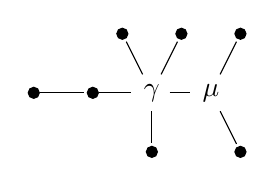
\begin{tikzpicture}	
      \tikzstyle{every edge}=[-,>=stealth',shorten >=1pt,auto,thin,draw]
		\node[basic] (A1) at (0, 0) {};
		\node[basic] (A2) at (0.5*\edgeunit, 0) {};
		\node[] (gam) at (1*\edgeunit, 0) {$\gamma$};
		\node[] (mu) at (1.5*\edgeunit, 0) {$\mu$};
		\node[basic] (A3) at (0.75*\edgeunit, 0.5*\edgeunit ) {};
		\node[basic] (A4) at (1.25*\edgeunit, 0.5*\edgeunit) {};
		\node[basic] (A5) at (1.75*\edgeunit, 0.5*\edgeunit) {};
		\node[basic] (A6) at (1.75*\edgeunit, -0.5*\edgeunit) {};
		\node[basic] (A7) at (1*\edgeunit, -0.5*\edgeunit) {};
		\path (A1) edge [] (A2)
        (A2) edge [] (gam)
        (gam) edge [] (mu)
        (gam) edge [] (A3)
        (gam) edge [] (A4)
        (gam) edge [] (A7)
        (mu) edge [] (A5)
        (mu) edge [] (A6);
	\end{tikzpicture}
&\hspace{1.5cm} &
 \hspace{0.5cm}
	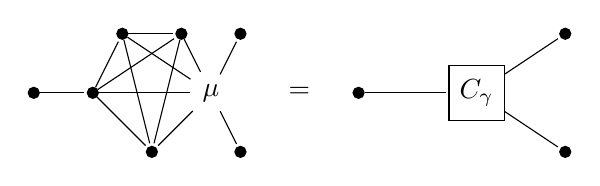
\begin{tikzpicture}	
      \tikzstyle{every edge}=[-,>=stealth',shorten >=1pt,auto,thin,draw]
		\node[basic] (A1) at (0, 0) {};
		\node[basic] (A2) at (0.5*\edgeunit, 0) {};
		\node[] (mu) at (1.5*\edgeunit, 0) {$\mu$};
		\node[basic] (A3) at (0.75*\edgeunit, 0.5*\edgeunit ) {};
		\node[basic] (A4) at (1.25*\edgeunit, 0.5*\edgeunit) {};
		\node[basic] (A5) at (1.75*\edgeunit, 0.5*\edgeunit) {};
		\node[basic] (A6) at (1.75*\edgeunit, -0.5*\edgeunit) {};
		\node[basic] (A7) at (1*\edgeunit, -0.5*\edgeunit) {};
		\node[] (eg) at (2.25*\edgeunit, 0*\edgeunit) {=};
		\path (A1) edge [] (A2)
        (A2) edge [] (mu)
        (A2) edge [] (A3)
        (A2) edge [] (A4)
        (A2) edge [] (A7)
        (A3) edge [] (A4)
        (A3) edge [] (mu)
        (A3) edge [] (A7)
        (A4) edge [] (mu)
        (A4) edge [] (A7)
        (mu) edge [] (A7)
        (mu) edge [] (A5)
        (mu) edge [] (A6);
		\node[basic] (A1b) at (2.75*\edgeunit, 0) {};
		\node[clique] (Cg) at (3.75*\edgeunit, 0) {$C_\gamma$};
		\node[basic] (A5b) at (4.5*\edgeunit, 0.5*\edgeunit) {};
		\node[basic] (A6b) at (4.5*\edgeunit, -0.5*\edgeunit) {};
		\path (A1b) edge [] (Cg)
        (Cg) edge [] (A5b)
        (Cg) edge [] (A6b);
	\end{tikzpicture}
\end{tabular}
 \caption{$a)$ Example of an original tree $T$. $b)$ Graph resulting from the marginalization of node $\gamma$ in $T$. Clique $C_\gamma$ appears, and is separated by nodes from the rest of the graph.}
 \end{center}
\end{figure}
Les séparateurs des cliques restent des noeuds, ce qui permet d'écrire :
$$|R_{\setminus \gamma} | = \prod_{\substack{kl \in T \\ \{k,l\} \neq \gamma }} (1- \rho_{kl}^2) \times |R_{C_\gamma}|$$

Si $T$ est marginalisé sur deux noeuds $\gamma$ et $\mu$ à la fois, une clique $C_{\gamma \mu}$ apparaît, formée par l'union des voisins des deux noeuds dans $T$. Ici $\gamma$ et $\mu$ sont liés dans $T$, sans quoi la corrélation partielle $c_{\gamma \mu}$ est nulle. Il est encore possible d'écrire :
$$| R_{\setminus \{\gamma,\mu\}}| = \prod_{\substack{kl \in T \\ \{k,l\} \notin \{\gamma,\mu\}}} (1-\rho_{kl}^2) \times |R_{C_{\gamma\mu}}|$$
Alors :
\begin{align*}
    \frac{|R|\;|R_{\setminus \{\mu\gamma\}}|}{|R_{\setminus\gamma}|\;|R_{\setminus \mu}|} &= \frac{ \prod_{kl\in T} (1-\rho_{kl}^2)\prod_{\substack{kl\in T\\ \{k,l\} \notin \{\mu, \gamma\}}} (1-\rho_{kl}^2)}{\prod_{\substack{kl\in T \\\{k,l\} \neq \gamma }} (1-\rho_{kl}^2)\prod_{\substack{kl\in T \\ \{k,l\} \neq \mu }} (1-\rho_{kl}^2)} \times \frac{|R_{C_{\gamma \mu}}|}{|R_{C_\gamma}||R_{C_\mu}|}\\
     &=(1-\rho_{\mu\gamma}^2)\times \frac{|R_{C_{\gamma \mu}}|}{|R_{C_\gamma}||R_{C_\mu}|}
\end{align*}
 On obtient:
 $$  c_{\mu\gamma}^2 = 1-(1-\rho_{\mu\gamma}^2)\times \frac{|R_{C_{\gamma \mu}}|}{|R_{C_\gamma}||R_{C_\mu}|} $$

\end{document}